% preamble
% report --> small books, reports, etc...
\documentclass{report}
% used to show subsubsections in the table of contents.
\setcounter{tocdepth}{4}
\setcounter{secnumdepth}{4}

% needed if we want to put images
\usepackage{graphicx}

% used to make the table of contents clickable
\usepackage{hyperref}
\hypersetup{
    colorlinks,
    citecolor=black,
    filecolor=black,
    linkcolor=black,
    urlcolor=black
}

%used to make tables
\usepackage{booktabs}
\usepackage{tabularx}

% let's change this ugly serif font!
\renewcommand{\familydefault}{\sfdefault}

% used to manage images
\usepackage{float}


% now start with the RASD document
\begin{document}
	\title{\textbf{myTaxiService} \\ -  \\ \textbf{Requirements Analysis and Specification Document}}
	\author{Davide Cremona, Simone Deola}
	\maketitle

	\tableofcontents

	
	\newpage
\chapter{Introduction}

	\section{Purpose}
	This document is the R.A.S.D. (Requirement Analysis and Specification Document).
	The purpose of this document is the description of the "myTaxiService" system. 
	At first, it will provide functional and non-functional requirements, a complete overview of the constraints of the system and its limits. Then it will explain in detail the dynamics of the system using real-life use cases.
	Finally this document will provide a base for the developers that concretely have to implement the system.

	\section{Actual System}
	The functionality that the new system will provide is now not supported. 
	So the entire system must be developed without using or modifying existing system.

	\section{Scope}
	The objective of “myTaxiService” is to provide an interface between \hyperref[sec:customer]{customers} and \hyperref[sec:tdriver]{taxi drivers} to optimize their interaction and provide a fair management of taxi queues. The \hyperref[sec:normaluser]{users}, once registered through the mobile application or the web application, can request a taxi for their travel or reserve one, specifying the origin and the destination. The reservation can be done at least two hour before the ride; if the reservation can take place, the system will allocate a taxi 10 minutes before the meeting time.
	On the other side, \hyperref[sec:tdriver]{taxi drivers} can inform the system that they are waiting for a client and accept or decline a ride request. If the request has been accepted, a notification will be sent to the requesting \hyperref[sec:customer]{customer} with the identification number of the incoming taxi and the time he has to wait. Otherwise, if the request has been rejected it will be forwarded to the next taxi in the queue.
	The system has to optimize the management of \hyperref[sec:customer]{customers} requests giving the rides to the taxi with the highest priority that has to be evaluated in function of avaiability and the nearness of the \hyperref[sec:tdriver]{taxi driver}.

	\section{Actors}
		\begin{itemize}
		  \item \textbf{Guest User:}\label{sec:normaluser} guest users are unlogged or unregistered users. They can visit the login page or the registration forms.

		  \item \textbf{Registered User:}\label{sec:ruser} this kind of user identify either a Guest User or a Taxi Driver.

		  \item \textbf{Customer:}\label{sec:customer} this kind of user is the end-user of the service. He can perform request for taxis or reserve a ride. In his personal page he can view his requests and the system responses.

		  \item \textbf{Taxi Driver:}\label{sec:tdriver} this kind of user is composed by the actual taxi drivers that can only see customers requests that has been forwarded by the system. He can accept or decline these requests. Also, he's considered a special kind of user because one can register as a "Taxi Driver" only if he provide a valid Taxi licence.
		\end{itemize}

	\section{Goals}

		\begin{itemize}
			\item \textbf{\lbrack G.1\rbrack}\label{sec:g1} Allow \hyperref[sec:normaluser]{guest user} to become a \hyperref[sec:customer]{customer} creating a myTaxiService Account.

			\item \textbf{\lbrack G.2\rbrack}\label{sec:g2} Allow \hyperref[sec:normaluser]{guest user} to become a \hyperref[sec:customer]{customer} using his Facebook Account.

			\item \textbf{\lbrack G.3\rbrack}\label{sec:g3} Allow \hyperref[sec:normaluser]{guest user} to become a \hyperref[sec:tdriver]{taxi driver}.

			\item \textbf{\lbrack G.4\rbrack}\label{sec:g4} Allow \hyperref[sec:ruser]{registered user} to log in with myTaxiService account.

			\item \textbf{\lbrack G.5\rbrack}\label{sec:g5} Allow \hyperref[sec:customer]{customer} to log in with Facebook account.

			\item \textbf{\lbrack G.6\rbrack}\label{sec:g5} Allow a \hyperref[sec:normaluser]{Registered User} to view or modify his username and email.

			\item \textbf{\lbrack G.7\rbrack}\label{sec:g7} Allow a \hyperref[sec:normaluser]{Registered User} to retrieve his password if he doesn't remember it.

			\item \textbf{\lbrack G.8\rbrack}\label{sec:g8} Allow a \hyperref[sec:normaluser]{RegisteredUser} to signal another one if he has made a bad use of the system.

			\item \textbf{\lbrack G.9\rbrack}\label{sec:g9} Allow \hyperref[sec:customer]{customers} to require a taxi.

			\item \textbf{\lbrack G.10\rbrack}\label{sec:g10} Allow \hyperref[sec:customer]{customers} to reserve a ride.

			\item \textbf{\lbrack G.11\rbrack}\label{sec:g11} Allow \hyperref[sec:customer]{customers} to delete a previous reservations.

			\item \textbf{\lbrack G.12\rbrack}\label{sec:g12} Allow \hyperref[sec:tdriver]{taxi drivers} to accept or decline a ride request.

			\item \textbf{\lbrack G.13\rbrack}\label{sec:g13} Allow \hyperref[sec:tdriver]{taxi drivers} to notify their availability.
		\end{itemize}
		
	\section{Definitions, Acronyms, Abbreviations}
		
		\subsection{Definitions}

		\subsection{Acronyms}
			\begin{itemize}
				\item RASD: Requirement Analysis and Specification Documents.
				\item DD: Design Document.
				\item UML: Unified Modeling Language.
				\item OS: Operative System.
				\item API: Application Program Interface.
				\item GPS: Global Positioning System.
				\item HTTP: Hypertext Transfer Protocol.
				\item HTTPS: Secure Hypertext Transfer Protocol.
			\end{itemize}

		\subsection{Abbreviations}
			\begin{itemize}
				\item G.x is the x-Goal
				\item Req.x is the x-Functional Requirement
				\item Dom.x is the x-Domain Assumption
			\end{itemize}
		
	\section{Reference documents}
		\begin{itemize}
			\item \href{http://www.math.uaa.alaska.edu/~afkjm/cs401/IEEE830.pdf}{(IEE830) IEEE Recommended Practice for Software Requirements Specifications}
		\end{itemize}
		
	\section{Document overview.}
	Until now, we have given a general explanation about the software functionalities and a brief description of this document. Now we will describe what the rest of this RASD contains.\\
	In Section 2 we will focus more on system constraints and assumptions.\\
	In Section 3 we will describe requirements, typical scenarios and use-cases. In this section there is also a collection of UML diagrams that describes in particular the functionalities of the system.\\
	//TODO SECTION 4
	\chapter{Overall Description}
	
	\section{Product perspective}
	The system will be composed of a web application and a mobile application developed for the three major OS ( Apple iOS, Android, Windows 10). The system will provide some API with the purpose of a future connection with another travel planning systems. 
		
	\section{User Characteristics}
	% this user here is ok and don't have to be hyperreferred
	The users that we suppose will use our system are of two types. the ones who want to find a taxi for a travel in the simplest way (\hyperref[sec:customer]{customers}). The others are \hyperref[sec:tdriver]{taxi drivers} that want to increment their productivity. The first ones must be able to access to a web browser or download and using a mobile application, the second ones also must have a taxi license.
		
	\section{Constrains}
		
		\subsection{Regulatory Policies}
		myTaxiService  has to meet regulatory policies about taxies in the countries where it will be used.

		\subsection{Hardware Limitations}
		The only hardware limitation that the myTaxiService mobile application has to meet will be the mobile phones characteristics. the rest of the system will be no affected by particular hardware limitations.

		\subsection{Software Limitations}
		myTaxiService mobile application has to be compatible with all major mobile operating systems (Android, Apple iOS, Windows 10).
		Also myTaxiService web application has to be compatible with all major browser (Chrome, Safari, Firefox, Microsoft Edge).

		\subsection{Parallel Operations}
		Our system must be able to perform parallel operations on the database to satisfy all the requests from multiple users.

		\subsection{Documents Related}

			\begin{itemize}
				\item Requirements and Analysis Specification Document (RASD)

				\item Design Document (DD)
			\end{itemize}

	\section{Assumptions}

			\begin{itemize}
				\item Every \hyperref[sec:tdriver]{taxi driver} has equipped a smartphone during working hours.

				\item Every \hyperref[sec:tdriver]{taxi driver} has a unique taxi license.

				\item Every taxi has a GPS locator to send GPS information to the central server.

				\item Android, Apple iOS or Windows 10 is avaiable on the \hyperref[sec:ruser]{registered users} smartphones.

				\item Every \hyperref[sec:ruser]{registered users} can be connected to the Internet with a mobile device when outside.

				\item When a \hyperref[sec:customer]{customer} require a taxi, the GPS informations about his location are automatically sended to the central server.

				\item The reservation of a ride is made at least two hours before the ride.

				\item Deletion of a reservation is made at least two hours before the ride.

				\item Requests from \hyperref[sec:customer]{customers} are automatically notified to the first \hyperref[sec:tdriver]{taxi driver} in the zone queue.

				\item If a \hyperref[sec:tdriver]{taxi driver} declines a request he will be placed in the bottom of the zone queue.

				\item If a request is declined it will be forwarded to the next \hyperref[sec:tdriver]{taxi driver} in the zone queue.

				\item If a \hyperref[sec:customer]{customer} make a bad use of the taxi request system, he can be reported as a bad \hyperref[sec:customer]{customer}.

				\item If a \hyperref[sec:tdriver]{taxi driver} notifies his availability is because he is actually avaiable

				\item If a \hyperref[sec:tdriver]{taxi driver} notifies his availability is because he wants to be notified of \hyperref[sec:customer]{customers} that needs a ride.

				\item If a \hyperref[sec:tdriver]{taxi driver} accept a request, the requesting \hyperref[sec:customer]{customer} will be notified
			\end{itemize}

	\section{Future possible Implementations}
	A possible future implementation can be a complex feedback system that permits to the \hyperref[sec:customer]{customers} to leave a comment about the \hyperref[sec:tdriver]{taxi driver} and vice versa.
	For example \hyperref[sec:tdriver]{taxi drivers} can be interested in knowing the punctuality or how is the behave of the \hyperref[sec:customer]{customer} that requests the ride.
	\chapter{Specific Requirements}
This chapter contains a detailed description of how the applications works and its features. It also gives a specification of the functional and quality requirements.

	%External Interface Requirements Section
	\documentclass[10pt]{article}
\usepackage[usenames]{color} %usato per il colore
\usepackage{amssymb} %maths
\usepackage{amsmath} %maths
\usepackage[utf8]{inputenc} %utile per scrivere direttamente in caratteri accentuati
\begin{document}
\[\section{External Interface Requirements}
	This section gives a description of the various inputs and relative outputs of the system. It also gives a description of the hardware, software and communication interfaces that are necessary to make the system work. It will also provide a generic visualization of the user interface in the various user platforms.

		\subsection{User Interfaces}
		Here we describe in particular how the application should look like either for mobile and web application. To make an easier explanation of the aspect of the various screen of the application we are going to use Mockup.
			\subsubsection{Login}
			On this page the users can log in with username and password or with Facebook (only if as registered user is a Customer). If the user is not already registered can access to the registration pages (for Customer or for Taxi Drivers). Also if the users forgot the password from this page can go to the forgot password page.
				
				\begin{figure}[H]
					\centering
					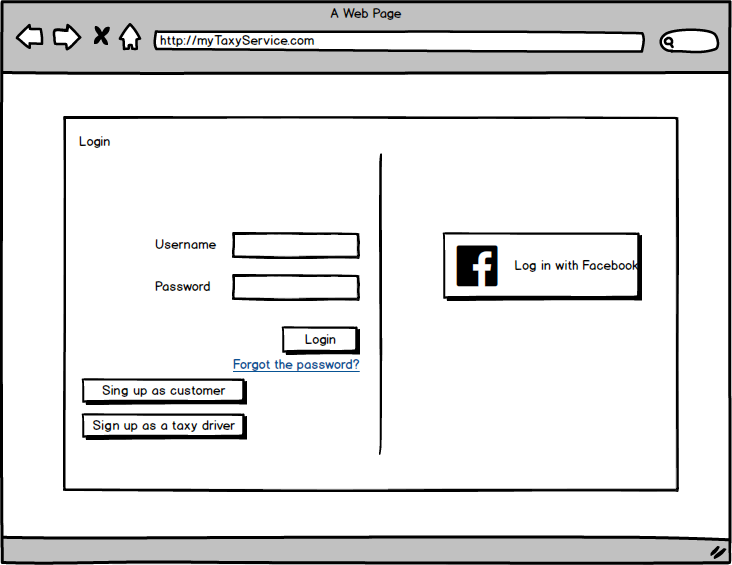
\includegraphics[scale=0.5]{IMG/UserInterfaces/CustomerLogin.png}
					\caption{Login Page, web version}\label{login_w}
				\end{figure}
				\begin{figure}[H]
					\centering
					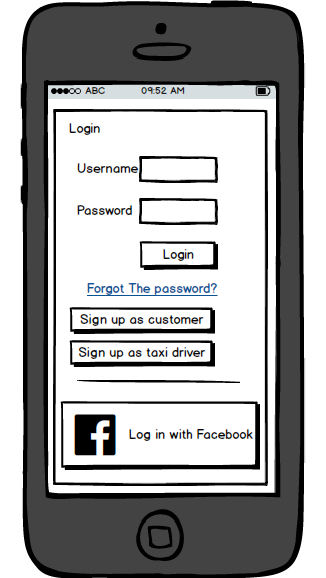
\includegraphics[scale=0.4]{IMG/UserInterfaces/CustomerLogin_m.png}
					\caption{Login Page, mobile version}\label{login_m}
				\end{figure}
			
			
			\subsubsection{Customer registration}
			On this page the users can register itself. This page must provide two way of registration, registration with the standard form ( e-mail, password and username) of with Facebook API.
			
				\begin{figure}[H]
					\centering
					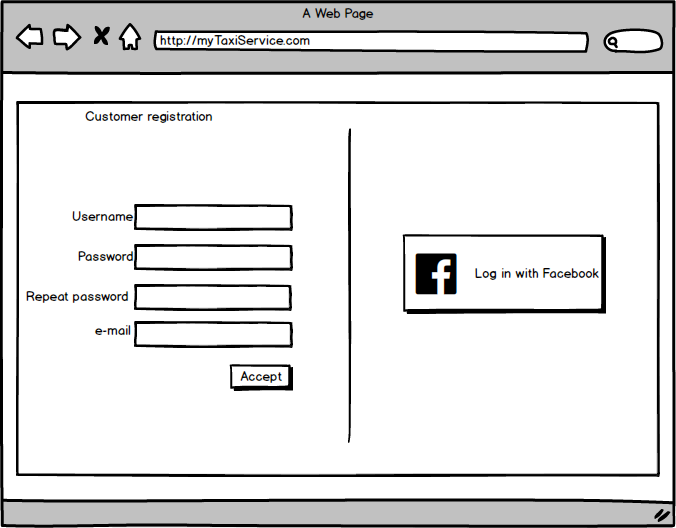
\includegraphics[scale=0.5]{IMG/UserInterfaces/CustomerRegistration.png}
					\caption{Customer registration Page, web version}\label{cregistration_w}
				\end{figure}
				\begin{figure}[H]
					\centering
					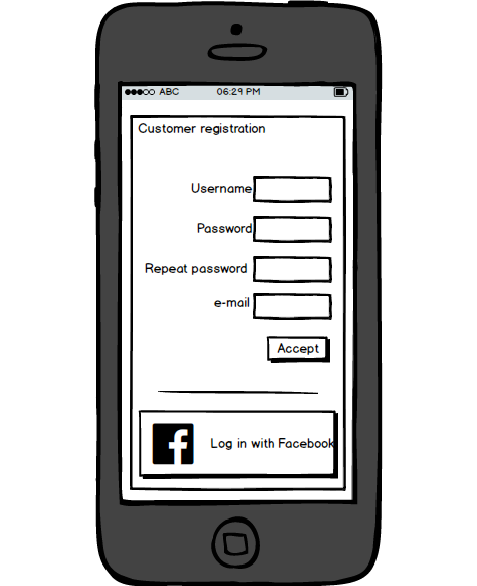
\includegraphics[scale=0.4]{IMG/UserInterfaces/CustomerRegistration_m.png}
					\caption{Customer registration Page, mobile version}\label{cregistration_m}
				\end{figure}
			
			\subsubsection{Taxi Drivers registration}
			On this page the users can register itself as a taxi driver. Taxi driver have a special form to been registered because of the additional information the user must provide (taxi license number). Just because the additional information the registration can be done just with the standard form.
				
				\begin{figure}[H]
					\centering
					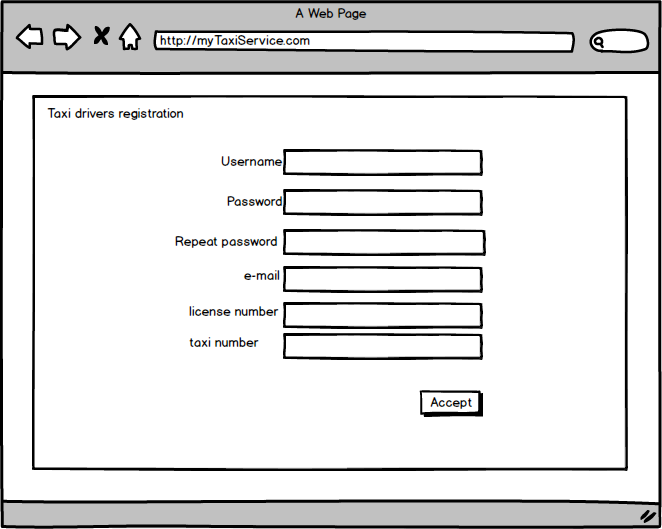
\includegraphics[scale=0.5]{IMG/UserInterfaces/TaxiDriverRegistration.png}
					\caption{Taxi Driver registration Page, web version}\label{tregistration_w}
				\end{figure}
				\begin{figure}[H]
					\centering
					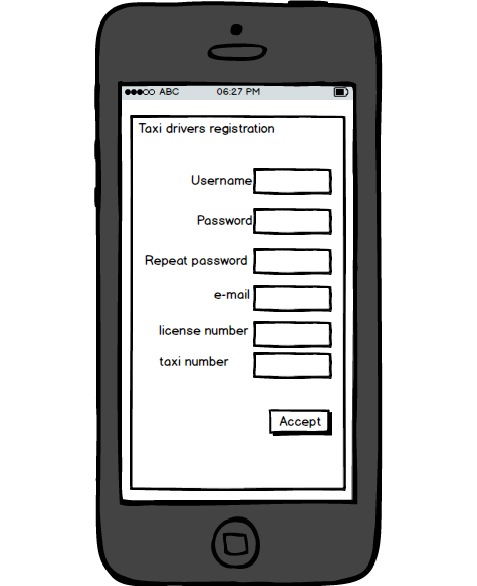
\includegraphics[scale=0.4]{IMG/UserInterfaces/TaxiDriverRegistration_m.png}
					\caption{Taxi Driver registration Page, mobile version}\label{tregistration_m}
				\end{figure}
			
			\subsubsection{Customer home page}
			On this page the Customer can see his position (information from his GPS) and perform all the main operation that he can perform. He can Request a taxi on the position showed, can go to the reservation page (in which can reserve a ride), can visit his personal page (in which can see all the information of his profile), can go to the information page (information about myTaxiService) or go to the 'my reservation page' (in which can manage all the previous reserved ride). 
			
				\begin{figure}[H]
					\centering
					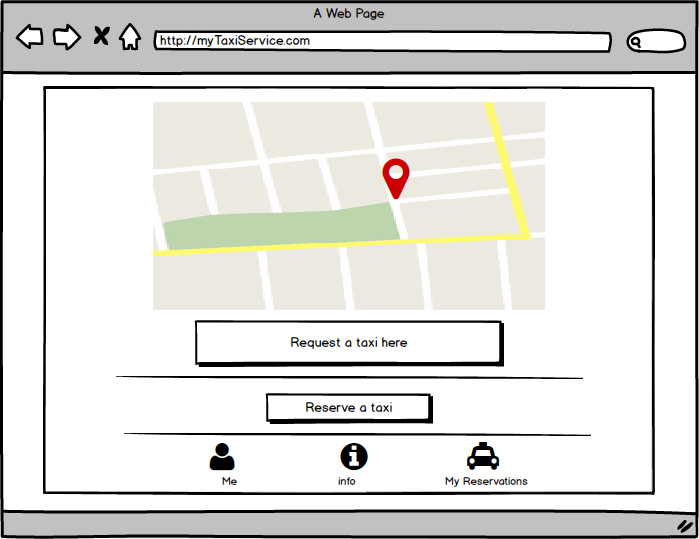
\includegraphics[scale=0.5]{IMG/UserInterfaces/mainCustomer.png}
					\caption{Customer home page, web version}\label{chome_w}
				\end{figure}
				\begin{figure}[H]
					\centering
					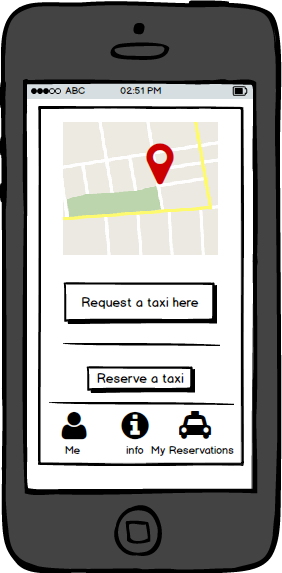
\includegraphics[scale=0.4]{IMG/UserInterfaces/mainCustomer_m.png}
					\caption{Customer home page, mobile version}\label{chome_m}
				\end{figure}
			
			\subsubsection{Reservation page}
			On this page the Customer can reserve a taxi ride. To do this he must insert a Origin position, a Destination position, a Data and a Time. The reservation must be at least two hours after the current Time, so the system must avoid to reserve a previous ride.
			
				\begin{figure}[H]
					\centering
					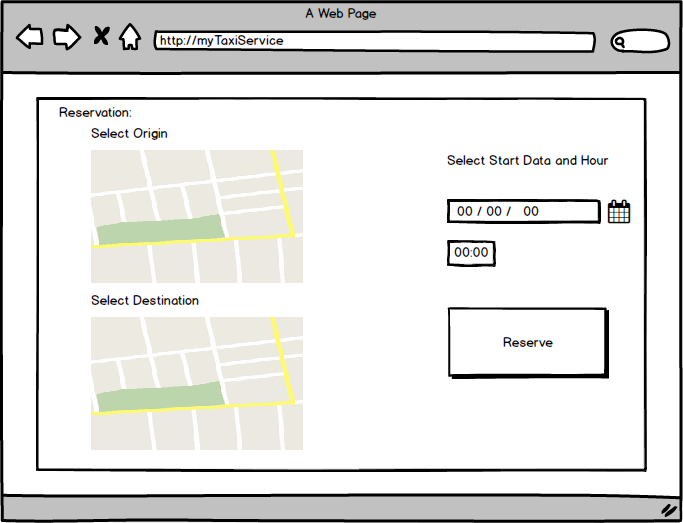
\includegraphics[scale=0.5]{IMG/UserInterfaces/reservationCustomer.png}
					\caption{Reservation page, web version}\label{reservation_w}
				\end{figure}
				\begin{figure}[H]
					\centering
					\includegraphics[scale=0.4]{IMG/UserInterfaces/reservationCustomer_m.png}
					\caption{Reservation page, mobile version}\label{reservation_m}
				\end{figure}
			
			\subsubsection{My reservation Page}
			On this page Customer can see all the reservation he have already done and adding some new. For each previous reservation can see all the information and, if the Date is before the next two hours, can delete it.			
			
				\begin{figure}[H]
					\centering
					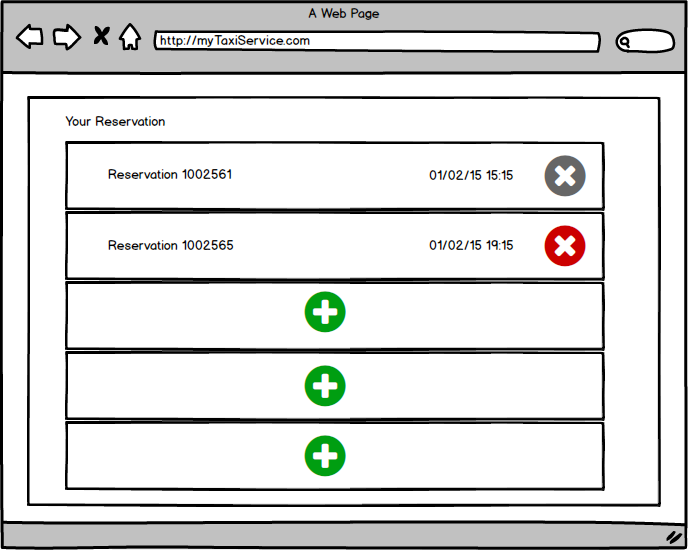
\includegraphics[scale=0.5]{IMG/UserInterfaces/myReservation.png}
					\caption{My reservation, web version}\label{myreservation_w}
				\end{figure}
				\begin{figure}[H]
					\centering
					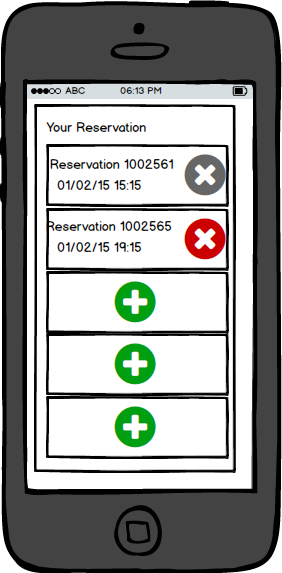
\includegraphics[scale=0.4]{IMG/UserInterfaces/myReservation_m.png}
					\caption{My reservation, mobile version}\label{myreservation_m}
				\end{figure}
			
			
			\subsubsection{Customer notification pop-up}
			This pop-up is showed to the requesting Customer when his request has been handled. On this pop-up the system show also the number of the incoming taxi and an approssimative waiting time.
			
				\begin{figure}[H]
					\centering
					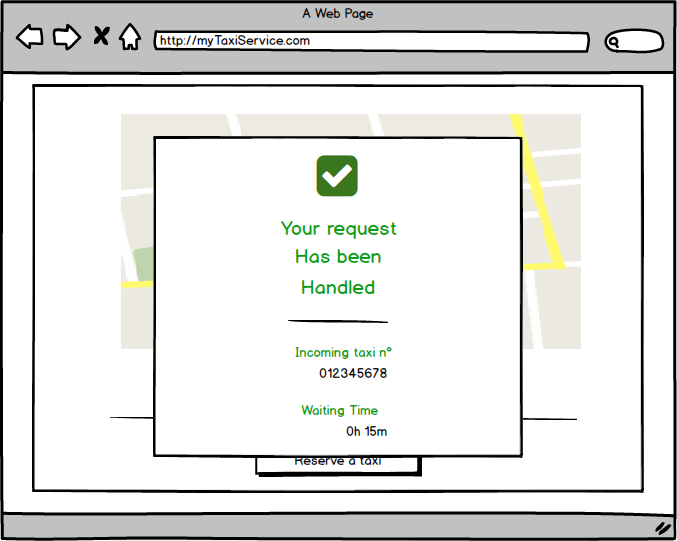
\includegraphics[scale=0.5]{IMG/UserInterfaces/customerNotification.png}
					\caption{Customer nofication, web version}\label{requestHandlded_w}
				\end{figure}
				\begin{figure}[H]
					\centering
					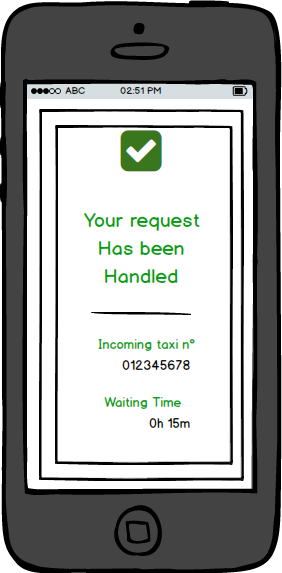
\includegraphics[scale=0.4]{IMG/UserInterfaces/customerNotification_m.png}
					\caption{Customer notification, mobile version}\label{requestHandled_m}
				\end{figure}
			
			\subsubsection{User page}
			This page show all the information about your user and show how many time you've been notified as bad user.
			
				\begin{figure}[H]
					\centering
					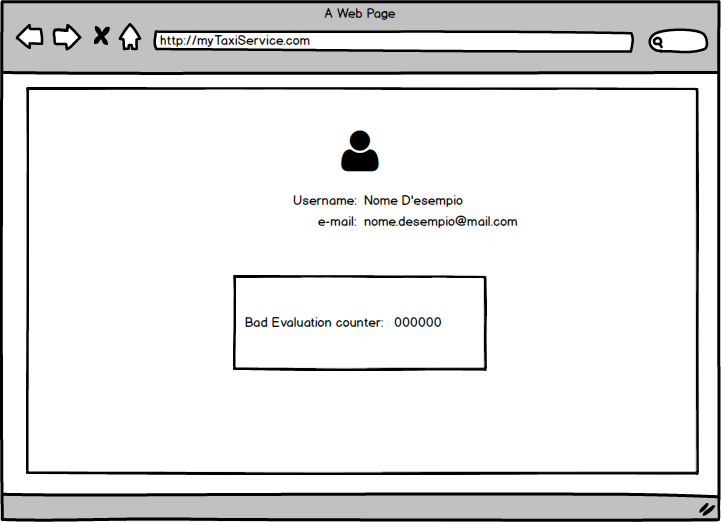
\includegraphics[scale=0.5]{IMG/UserInterfaces/userPage.png}
					\caption{User Page, web version}\label{cpersonalPage_w}
				\end{figure}
				\begin{figure}[H]
					\centering
					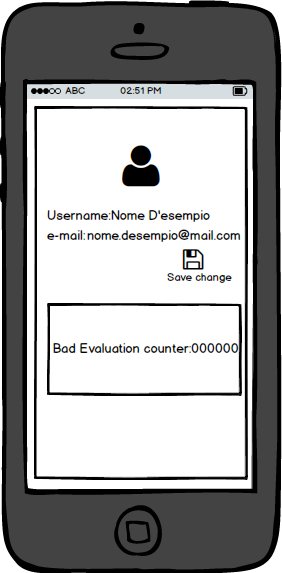
\includegraphics[scale=0.4]{IMG/UserInterfaces/userPage_m.png}
					\caption{User Page, mobile version}\label{cpersonalPage_m}
				\end{figure}

			
			\subsubsection{Taxi Driver home page}
			On this page the Taxi driver can see his position (information from his GPS) and inform the system about his availability.
			
				\begin{figure}[H]
					\centering
					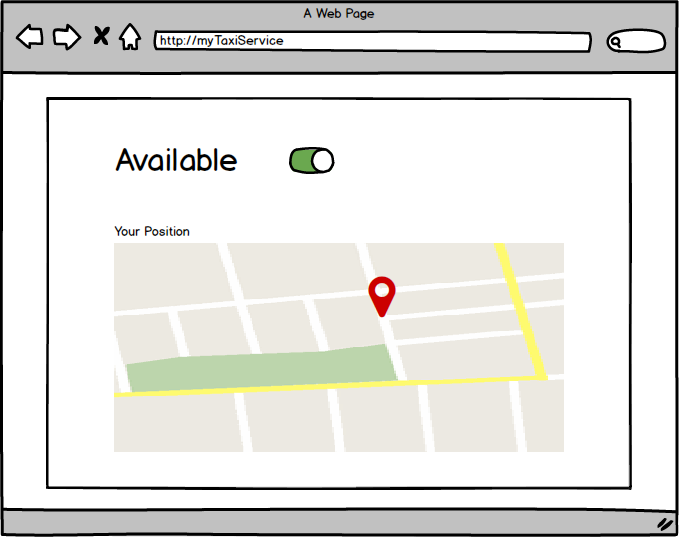
\includegraphics[scale=0.5]{IMG/UserInterfaces/mainTaxiDriver.png}
					\caption{Taxi driver home page, web version}\label{thomePage_w}
				\end{figure}
				\begin{figure}[H]
					\centering
					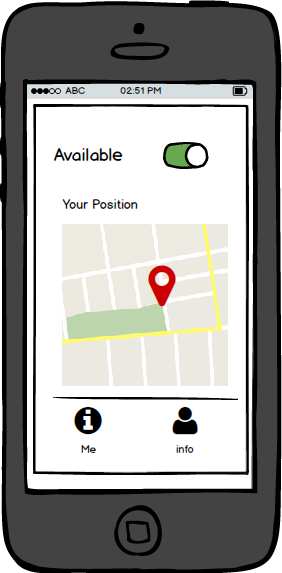
\includegraphics[scale=0.4]{IMG/UserInterfaces/mainTaxiDriver_m.png}
					\caption{Taxi driver home page, mobile version}\label{thomePage_m}
				\end{figure}
			
			
			
			\subsubsection{Taxi Driver notification}
			On this pop-up the taxi driver will notified of a request that he can handle. On this pop-up is showed also two button, with which the taxi driver can accept or decline the request.
			
				\begin{figure}[H]
					\centering
					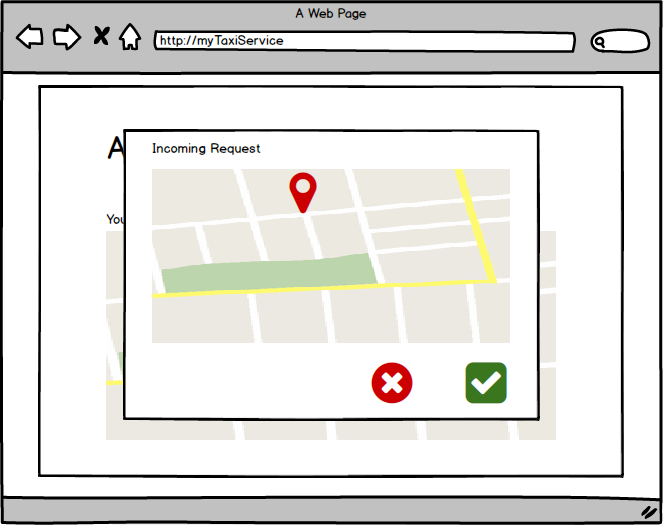
\includegraphics[scale=0.5]{IMG/UserInterfaces/notificationTaxiDriver.png}
					\caption{Taxi driver notification pop-up, web version}\label{requestNotification_w}
				\end{figure}
				\begin{figure}[H]
					\centering
					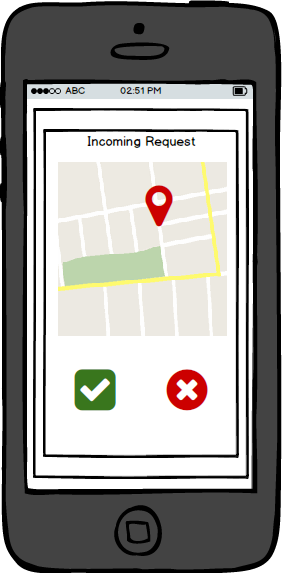
\includegraphics[scale=0.4]{IMG/UserInterfaces/notificationTaxiDriver_m.png}
					\caption{Taxi driver notification pop-up, mobile version}\label{requestNotification_m}
				\end{figure}
				
			
			\subsubsection{Registered user end ride page}
			When a taxi driver accept a ride this page is showed up to each registered user involved in this ride. On this page the taxi driver can check the name of the customer and the Origin position of his journey. When the ride is ended each of the registered user can give a bad evaluation to the other or simply end the ride and return to the main page.
				
				\begin{figure}[H]
					\centering
					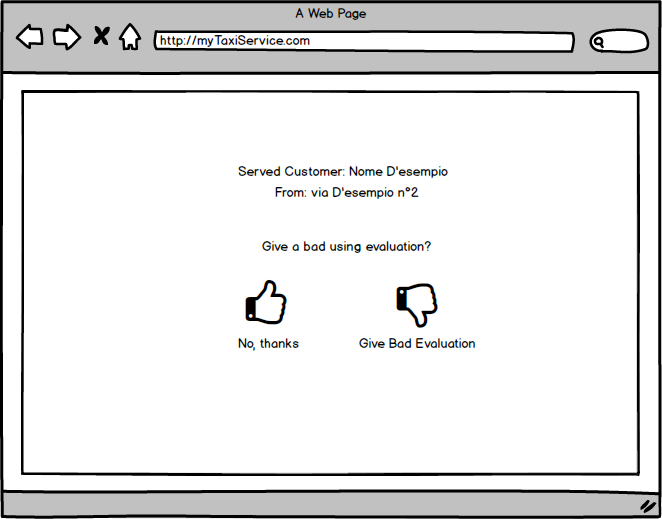
\includegraphics[scale=0.5]{IMG/UserInterfaces/onRidePage.png}
					\caption{On Ride Page, web version}\label{tendRidePage_w}
				\end{figure}
				\begin{figure}[H]
					\centering
					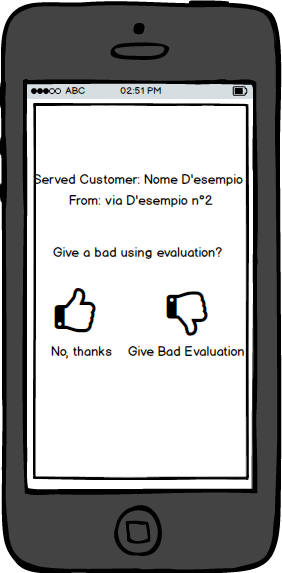
\includegraphics[scale=0.4]{IMG/UserInterfaces/onRidePage_m.png}
					\caption{On Ride page, mobile version}\label{tendRidePage_m}
				\end{figure}
				

		\subsection{Hardware Interfaces}
		Since mobile and web applications don't have any dedicated hardware we have not designed any hardware interfaces for our system.
		The interaction with the central database is performed by connections handled by the already installed operating system on the mobile devices or the users computers.

		\subsection{Software Interfaces}
			\begin{itemize}
				\item The mobile application communicates with the GPS application in order to get geographical informations about the user.
				
				\item The web application communicates with the browser in order to get geographical informations about the user.
				
				\item Mobile and web applications communicates with the database through HTTP requests to the server.
			\end{itemize}

		\subsection{Interfaces to Others Application}
			\begin{itemize}
				\item myTaxiService web application require that at least one of these browsers is installed on the user Personal Computer:
			
					\begin{center}
						\begin{table}[h!]
							
							\begin{center}
								\caption{Browsers}
								\label{tab:browsersTable}

								\begin{tabular}{cccc}
									\toprule
									\textbf{Name} & \textbf{Version} & \textbf{Company} & \textbf{Source}\\
									\midrule
									Safari & 9.0.1 & Apple Inc. & \href{http://www.apple.com/safari/}{Get Safari}\\
									\midrule
									Firefox & 41.0 & Mozilla & \href{https://www.mozilla.org/en-US/firefox/new/}{Get Firefox}\\
									\midrule
									Chrome & 46.0.2490 & Google & \href{https://www.google.com/chrome/browser/desktop/}{Get Chrome}\\
									\midrule
									Microsofr Edge & 20.10240.16384.0 & Microsoft & \href{https://www.microsoft.com/en-us/download/details.aspx?id=48126}{Get Edge}\\
									\bottomrule
								\end{tabular}
							\end{center}
							
						\end{table}
					\end{center}

				\item myTaxiService mobile application require that at least one of these operating systems is installed on the user Smartphone:

					\begin{center}
						\begin{table}[h!]
							
							\begin{center}
								\caption{Mobile Operative Systems}
								\label{tab:mobileOSTable}

								\begin{tabular}{cccc}
									\toprule
									\textbf{Name} & \textbf{Version} & \textbf{Company} & \textbf{Source}\\
									\midrule
									Android & KitKat 4.4W.2 or later & Google & \href{https://www.android.com}{Android Info}\\
									\midrule
									iOS & 9.1 or later & Apple Inc. & \href{http://www.apple.com/ios/}{iOS Info}\\
									\midrule
									Windows 10 & 10.0.10572.0 or later & Microsoft & \href{http://www.microsoft.com/it-it/mobile/windows10/?dcmpid=omc-org-globalsite.globalredirect}{Windows 10 Info}\\
									\bottomrule
								\end{tabular}
							\end{center}
							
						\end{table}
					\end{center}

				\item To give an additional LogIn method, we use also the "LogIn with Facebook" API relased by Facebook. Facebook Login for Apps is a fast and convenient way for people to create accounts and log into our system across multiple platforms. It is well described at \href{https://developers.facebook.com/docs/facebook-login}{Facebook Login API Page.}
			\end{itemize}


		\subsection{Communication Interfaces}
		The communication between system pieces is not specified because it is handled by the underlying operating systems for both the mobile application and the web portal.

		In particular, the web and mobile applictaions will communicate with the server through HTTP/HTTPS requests. 

			\begin{itemize}
				\item HTTP communicate through the port number 80 and is handled by the operating system. 
				\item HTTPS communicate through the port number 443 and is handled by the operating system.
			\end{itemize}\]
\end{document}
	
	%Functional Requirements Section
	\section{Functional Requirements}
	In this section are described, for every Actor, the Functional Requirements needed to reach the linked Goal.

		\subsection{Functional Requirements for Guest Users}
		Here are listed all the Functional Requirements referring to the Goals that affects Guest Users.

			\subsubsection{\lbrack \hyperref[sec:g1]{G.1 - Allow guest users to become a customer creating a myTaxiService Account}\rbrack}\label{sec:frs1}
			To allow the guest user to perform a successful registration the system has to:

				\begin{itemize}
					\item \lbrack Req.1\rbrack \label{sec:fr1_g1} provide a registration page containing:
						\begin{enumerate}
							\item A text box where the user can insert his username.
							\item Two text box where the user can insert his password (the second one is for security check).
							\item A text box where the user can insert his email. 
							\item A button to submit informations to the system.
						\end{enumerate}
					\item \lbrack Req.2\rbrack \label{sec:fr2_g1} The registration page shall be the only page accessible by a Guest User.
					\item \lbrack Req.3\rbrack \label{sec:fr3_g1} All the informations submitted by the user must be validated by the system.
					\item \lbrack Dom.1\rbrack \label{sec:da1_g1} The email used by the Guest User is a valid one.
				\end{itemize}

			\subsubsection{\lbrack \hyperref[sec:g2]{G.2 - Allow a Guests User to become a Customer using his Facebook Account}\rbrack}\label{sec:frs2}
			To allow the guest user to perform a successful registration using Facebook API, the system has to:

				\begin{itemize}
					\item \lbrack Req.1\rbrack \label{sec:fr1_g2} provide a registration page containing:
						\begin{enumerate}
							\item A button that calls the Facebook Registration API.
						\end{enumerate}
					\item \lbrack Req.2\rbrack \label{sec:fr2_g2} The registration page shall be the only page accessible by a Guest User.
					\item \lbrack Req.3\rbrack \label{sec:fr3_g2} All the informations must be evaluated by the Facebook system.
				\end{itemize}

			\subsubsection{\lbrack \hyperref[sec:g3]{G.3 Allow guest users to become a taxi driver}\rbrack}\label{sec:frs3}
			To allow the guest user to become a Taxi Driver, the system must:

			%"^\w+@[a-zA-Z_]+?\.[a-zA-Z]{2,3}$"

				\begin{itemize}
					\item \lbrack Req.1\rbrack \label{sec:fr1_g3} provide a registration page containing:
						\begin{enumerate}
							\item A text box where the user can insert his username.
							\item Two text box where the user can insert his password (the second one is for security check).
							\item A text box where the user can insert his email.
							\item A text box where the user can insert his valid taxi license.
							\item A text box where the user can insert his valid taxi number.
							\item A button to submit informations to the system.
						\end{enumerate}
					\item \lbrack Req.2\rbrack \label{sec:fr2_g3} The registration page shall be the only page accessible by a Guest User.
					\item \lbrack Req.3\rbrack \label{sec:fr3_g3} All the informations submitted by the Guest User must be validatedby the system.
					\item \lbrack Dom.1\rbrack \label{sec:da1_g3} The email used by the Guest User is a valid one.
				\end{itemize}

		\subsection{Functional Requirements for Registered Users}
		Here are listed all the Functional Requirements referring to the Goals that affects Registered Users.

			\subsubsection{\lbrack \hyperref[sec:g4]{G.4 Allow registered users to log in with myTaxiService account.}\rbrack}\label{sec:frs4}
			To allow a registered user to log in with his myTaxiService account, the system must:

				\begin{itemize}
					\item \lbrack Req.1\rbrack \label{sec:fr1_g4} provide a login page containing:
						\begin{enumerate}
							\item A text box where the user can insert his username.
							\item A text box there the user can insert his password.
							\item A button to submit informations to the system.
						\end{enumerate}
				\end{itemize}

			\subsubsection{\lbrack \hyperref[sec:g5]{G.5 Allow a Registered User to view or modify his username and email.}\rbrack}\label{sec:frs5}
			To allow a Registered User to view or modify his username and email, the system must:

				\begin{itemize}
					\item \lbrack Req.1\rbrack \label{sec:fr1_g5} provide an homepage that contains:
						\begin{enumerate}
							\item A button that, if clicked, shows the page that contains the Registered User's informations.
						\end{enumerate}
					\item \lbrack Req.2\rbrack \label{sec:fr2_g5} provide a page used to show Registered User's informations that contains:
						\begin{enumerate}
							\item A clickable label showing the username of the Registered User.
							\item A clickable label showing the email of the Registered User.
							\item A box with a label inside that shows how many times the Registered User has been reported as a bad user.
						\end{enumerate}
					\item \lbrack Req.3\rbrack \label{sec:fr3_g5} The personal Registered User's page shall be only accessible after the login.
				\end{itemize}

			\subsubsection{\lbrack \hyperref[sec:g6]{G.6 Allow a Registered User to retrieve his password if he doesn't remember it.}\rbrack}\label{sec:frs6}
			To allow a Registered User to retrieve his password, the system must:

				\begin{itemize}
					\item \lbrack Req.1\rbrack \label{sec:fr1_g6} on the log in page, provide a link that will show to the Registered User a field where he can write his email to allow the system to send him an email containing the password.
				\end{itemize}

			\subsubsection{\lbrack \hyperref[sec:g7]{G.7 Allow a Registered User to signal another one if he has made a bad use of the system.}\rbrack}\label{sec:frs7}
			To allow a Registered User to signal another one, the system must:

				\begin{itemize}
					\item \lbrack Req.1\rbrack \label{sec:fr1_g7} check if the Registered User is correctly logged in.
					\item \lbrack Req.2\rbrack \label{sec:fr2_g7} for Taxi Drivers, provide an end-ride page that contains:
						\begin{enumerate}
							\item A label showing the username of the Customer that he has just served.
							\item A label showing the starting location of the current ride.
							\item A label that asks to the Taxi Driver if he want to report the Customer.
							\item A button that ends the current ride without reporting the Customer.
							\item A button that ends the current ride increments the Customer's Bad Evaluation Counter.
						\end{enumerate}
					\item \lbrack Req.3\rbrack \label{sec:fr3_g7} When one of the Taxi Driver end-ride page button is pressed, the system must ensure that the page is not reachable anymore and the Taxi Driver must access only to his homepage.
					\\
					\item \lbrack Req.4\rbrack \label{sec:fr4_g7} for Customers, provide an end-ride page that contains:
						\begin{enumerate}
							\item A label showing the username of the Taxi Driver that has just served him.
							\item A label showing the starting location of the current ride.
							\item A label that asks to the Customer if he want to report the Taxi Driver.
							\item A button that ends the current ride without reporting the Taxi Driver.
							\item A button that ends the current ride and increments the Taxi Driver's Bad Evaluation Counter.
						\end{enumerate}
					\item \lbrack Req.5\rbrack \label{sec:fr5_g7} When one of the Customer end-ride page button is pressed, the system must ensure that the page is not reachable anymore and the Customer must access only to his homepage.
					\item \lbrack Req.6\rbrack \label{sec:fr6_g7} The end-ride page shall be only accessible after the Registered User login.
					\item \lbrack Dom.1\rbrack \label{sec:da1_g7} The ride is ended after a Taxi Driver or a Customer action.
				\end{itemize}

		\subsection{Functional Requirements for Customers}
		Here are listed all the Functional Requirements referring to the Goals that affects Customers.

			\subsubsection{\lbrack \hyperref[sec:g8]{G.8 Allow customers to log in with Facebook account.}\rbrack}\label{sec:frs8}
			To allow a customer to log in with Facebook account, the system must:

				\begin{itemize}
					\item \lbrack Req.1\rbrack \label{sec:fr1_g8} provide a button that calls the Facebook Login API.
					\item \lbrack Req.2\rbrack \label{sec:fr2_g8} delegate to the Facebook system all the checks about the existence of the user.
				\end{itemize}

			\subsubsection{\lbrack \hyperref[sec:g9]{G.9 Allow customers to require a taxi.}\rbrack}\label{sec:frs9}
			To allow the customers to require a taxi, the system must:

				\begin{itemize}
					\item \lbrack Req.1\rbrack \label{sec:fr1_g9} provide an homepage that contains:
						\begin{enumerate}
							\item A map showing the current location of the customer.
							\item A button that calls the function of the system to require a taxi (called "require button").
						\end{enumerate}
					\item \lbrack Req.2\rbrack \label{sec:fr2_g9} The require-taxi page shall be only accessible by Customers and after they have performed the login as a Customer.
				\end{itemize}

			\subsubsection{\lbrack \hyperref[sec:g10]{G.10 Allow customers to reserve a ride.}\rbrack}\label{sec:frs10}
			To allow the customers to reserve a ride, the system must:

				\begin{itemize}
					\item \lbrack Req.1\rbrack \label{sec:fr1_g10} provide an homepage that contains:
						\begin{enumerate}
							\item A button that, if clicked, shows the page used to reserve a ride.
						\end{enumerate}
					\item \lbrack Req.2\rbrack \label{sec:fr2_g10} provide a page used to reserve a ride that contains:
						\begin{enumerate}
							\item A map where the customer can select the starting location for his ride.
							\item A map where the customer can select the ending location for his ride.
							\item A field where the customer can insert the starting date for the ride.
							\item A field where the customer can insert the starting time for the ride.
							\item A button that calls the function of the system to reserve a ride (called "reserve button").
						\end{enumerate}
					\item \lbrack Req.3\rbrack \label{sec:fr3_g10} The page used to reserve a ride shall be only accessible after the Customer login.
					\item \lbrack Req.4\rbrack \label{sec:fr4_g10} "reserve button" must be clickable if and only if the reserve date and time is at least two hours after the current time. (for instance: if the current date is 10/10/2015 and current time is 10.00, the reservation time must be at least 12.00 of the 10/10/2015).
					\item \lbrack Req.5\rbrack \label{sec:fr5_g10} The system must notify the Customer that a Taxi Driver has accepted his reservation at least 10 minutes before the ride.
				\end{itemize}

			\subsubsection{\lbrack \hyperref[sec:g11]{G.11 Allow customers to delete a previous reservations.}\rbrack}\label{sec:frs11}
			To allow a customer to delete a previous reservation, the system must:

				\begin{itemize}
					\item \lbrack Req.1\rbrack \label{sec:fr1_g11} provide an homepage that contains:
						\begin{enumerate}
							\item A button that, if clicked, shows the page that contains all the reservations made by the customer.
						\end{enumerate}
					\item \lbrack Req.2\rbrack \label{sec:fr2_g11} provide a page that contains all the reservations made by the customer:
						\begin{enumerate}
							\item All reservations that have a difference between the start time and the current time of less than two hours are not erasable
							\item Other reservations are erasable.
							\item The page also contains a button to add a new reservation. If clicked that button leads the customer to the page used to reserve a ride (described in the Functional Requirements \hyperref[sec:fr3_g4]{Req.3 of G.4})
						\end{enumerate}
					\item \lbrack Req.3\rbrack \label{sec:fr3_g11} The page that contains all the reservations shall be only accessible after the Customer login.
					\item \lbrack Dom.1\rbrack \label{sec:da1_g11} The reservation is deleted after the Customer action.
				\end{itemize}

		\subsection{Functional Requirements for Taxi Drivers}
		Here are listed all the Functional Requirements referring to the Goals that affects Taxi Drivers.

			\subsubsection{\lbrack \hyperref[sec:g12]{G.12 Allow Taxi Drivers to accept or decline a ride request.}\rbrack}\label{sec:frs12}
			To allow Taxi Drivers to accept or decline ride requests, the system must:

			%The Taxi Driver must be already registered and logged in with a myTaxiService account.

				\begin{itemize}
					\item \lbrack Req.1\rbrack \label{sec:fr1_g12} notify the Taxi Driver (if he's available) that is at the top of the zone-queue that a new taxi-request is made \hyperref[sec:fr4_g9]{(Req.4 of G.9)}.
					\item \lbrack Req.2\rbrack \label{sec:fr2_g12} on the notification screen, show two buttons: one for theacceptance and one for the declination of the taxi-request.
				\end{itemize}


			\subsubsection{\lbrack \hyperref[sec:g13]{G.13 Allow Taxi Drivers to notify their availability.}\rbrack}\label{sec:frs13}
			To allow Taxi Drivers to notify their availability, the system must:
				\begin{itemize}
					\item \lbrack Req.1\rbrack \label{sec:fr1_g13} provide an home page that contains:
						\begin{enumerate}
							\item An ON/OFF button that signals to the system that the Taxi Driver is Available/Not Available.
							\item A map showing his current zone and position.
						\end{enumerate}
					\item \lbrack Req.1\rbrack \label{sec:fr1_g13} The home page should be accessible only if the Taxi Driver is logged in.
				\end{itemize}

	%Scenarios Section
	\section{Scenarios}
	Here are described in natural language some useful scenarios that shows how the system should work in different cases:

		\subsection{S.1 Registration as a Customer creating a myTaxiService account}\label{sec:NormalCustomerRegistrationScenario}
		To read the Functional Requirements for this scenario, refer to \hyperref[sec:frs1]{G.1 Functional Requirements Specification}\\

		Aristotle is new in the system and he wants to simplify the way he calls for a taxi. So he download the "myTaxiService" application from the Play Store (since he has a smartphone with the fancy Android 5.0 Lollipop Operative System) and he open it.
		The application shows to Aristotle the login screen and he taps on the "Sign Up as a Customer" button (see \hyperref[login_m]{Login Screen}) going to the registration page. In that page, he has to fill the form (see \hyperref[cregistration_m]{Customer Registration Screen (Mobile)}) and after that he clicks on the "Accept" button. If the data entered by Aristotle are ok, he is automatically logged in and he can start using myTaxiService. Otherwise, he is redirected to an error page, that describes what is the problem. 

		\subsection{S.2 Registration as a Customer using a Facebook Account}\label{sec:FacebookCustomerRegistrationScenario}
		To read the Functional Requirements for this scenario, refer to \hyperref[sec:frs2]{G.2 Functional Requirements Specifications}\\

		Pythagoras is new in the system and he wants to simplify the way he calls for a taxi, but he doesn't want to loose time inserting his credential into a boring registration form, so he decide to register with his Facebook Account.
		He download the application from the Apple App Store (since he has a glorious iPhone 6 Plus) and he open it.
		The application shows to Pythagoras the login screen and he taps on the "Log in With Facebook" button calling the Facebook Login API.
		If the registration is successful, the Facebook System will reply with the informations about the user and the myTaxiService system can create a record in the database with Pythagoras informations. Otherwise, he is redirected to an error page, that describes what is the problem.

		\subsection{S.3 Registration as a Taxi Driver creating a new Taxi Driver myTaxiService account.}\label{sec:TaxiDriverRegistrationScenario}
		To read the Functional Requirements for this scenario, refer to \hyperref[sec:frs3]{G.3 Functional Requirements Specifications}\\

		Thales is a great taxi worker and he wants to improve his service to the customers so he decide to join myTaxiService.
		First of all he visit the myTaxiService web page from his pc. That page shows the login screen (see \hyperref[login_m]{Login Screen}) and he clicks on the "Sign up as a Taxi Driver" button. The web application redirect him to the Taxi Drivers registration page. Thales fills up the form (see \hyperref[tregistration_w]{Taxi Driver Registration Screen (Web)}) and clicks on the "Accept" button. The system perform a special check for the validity of the given taxi licence and taxi number. If the data entered by Thales are ok, he is automatically logged in and he can start using myTaxiService as a Taxi Driver. Otherwise, he is redirected to an error page, that describes what is the problem.

		\subsection{S.4 Login with a myTaxiService account.}\label{sec:RegisteredUserLoginScenario}
		To read the Functional Requirements for this scenario, refer to \hyperref[sec:frs4]{G.4 Functional Requirements Specifications}\\

		Epicurus is a Registered User and he wants to login to use the myTaxiServer Application with his smartphone. So he taps on the application icon and start using it. myTaxiService Application shows to him the login screen (see \hyperref[login_m]{Login Screen}) and Epicurus fills up the form with his credentials. After that he submits the data by pressing the "Login" button. The Application calls the server function to check the credentials of Epicurus and if them are ok, the server reply to the application with a success message and the homepage is shown to Epicurus. Otherwise the server reply with an error message that is shown to Epicurus.

		\subsection{S.5 Customer Login with Facebook}
		To read the Functional Requirements for this scenario, refer to \hyperref[sec:frs5]{G.5 Functional Requirements Specifications}\\

		\label{sec:CustomerFacebookLoginScenario}
		Solon is a Customer of myTaxiService and he's registered with his Facebook account as described in the scenario \hyperref[sec:FacebookCustomerRegistrationScenario]{S.2}. Now he wants to log in and use myTaxiService from his iPhone.
		First of all he opens the application that shows the login screen (see \hyperref[login_m]{Login Screen}). In a second moment, he clicks on the "Log in with Facebook" button and he logs in.

		\subsection{S.6 Profile Modification.}\label{sec:RegisteredUserProfileModificationScenario}
		To read the Functional Requirements for this scenario, refer to \hyperref[sec:frs6]{G.6 Functional Requirements Specifications}\\

		Zeno is a Registered User but he wants to change his username. He open his browser and navigates to the myTaxiService Web Application. He logs in to the system and the application shows his homepage (see \hyperref[chome_m]{Homepage}). Zeno clicks on the "Me" button to view the profile page (see \hyperref[cpersonalPage_m]{Profile Page}). He clicks on his username to modify it. Once he is satisfied of his new username, he clicks on the "Save" button to save his modifications. Now Zeno is happy.

		\subsection{S.7 Password Retrieval}\label{sec:PasswordRetrievalScenario}
		To read the Functional Requirements for this scenario, refer to \hyperref[sec:frs7]{G.7 Functional Requirements Specifications}\\

		Archimedes is a Registered User and he wants to log in to the myTaxiService Application. Unfortunately, he doesn't remember his password, so he taps on the link in the login page (see \hyperref[login_m]{Login Screen}) and the myTaxiService system sends him an email with the password if the provided email is registered. Otherwise an error message is shown to Archimedes.

		\subsection{S.8 Reporting Abuses}\label{sec:ReportingAbusesScenario}
		To read the Functional Requirements for this scenario, refer to \hyperref[sec:frs8]{G.8 Functional Requirements Specifications}\\

		\label{sec:TaxiDriverReportingScenario}
		Crates is a Customer and he desperately wants to go to the cinema with his friends. He logs in to the myTaxiService Mobile Application and navigates to the homepage. Then he taps on the "Request a Taxi here" button and waits for a taxi (since he received the acceptance notification). But this taxi does not arrive and he can't reach the cinema in time. Crates is very frustated so he reports the Taxi Driver that has accepted his taxi request.
		\\
		\\
		\label{sec:CustomerReportingScenario}
		Gorgias is a Taxi Driver and he has already logged in to the myTaxiService Mobile Application and signaled his availability. He receives a taxi request from a Customer and he accept it. But when he goes to the meeting location, the Customer is not there. Gorgias has lost precious time and money so he is very hungry and reports the Customer through the application. 
		
		\subsection{S.9 Require a Taxi}\label{sec:TaxiRequiringScenario}
		To read the Functional Requirements for this scenario, refer to \hyperref[sec:frs9]{G.9 Functional Requirements Specifications}\\
		Plutarch is a Customer that want to go to his vacation house but he is already arrive to the city train station and he don't have a car, so he decide to call a taxi. He launch myTaxiService and the application show to him the homepage. He first check that the position showed is his current position so he tap the "Request a taxi here" button and wait for a taxi accept his request. After 2 min a Taxi Driver accept his request and a pop up notification notify it to Plutarch. The notification says that a taxi will reach his position after 10 min and informs Plutarch about the number of the incoming taxi, so Plutarch can't takes the Wrong taxi.
		
		

	%UML Models Section
	\section{UML Models}

		\subsection{Use-Case Diagrams}

		\subsection{Class Diagrams}

			\subsubsection{Registration through the creation of a new myTaxiService account.}
			To accompany this diagram, read the Scenario \hyperref[sec:NormalCustomerRegistrationScenario]{S.1}.

				\begin{table}[htpb]
					\centering
					\label{tab:NormalCustomerRegistrationDiagramTable}
					\begin{tabularx}{\textwidth}{lp{9cm}}
						\hline
						\hline
							\textbf{Subject}
						& 
							\textbf{Description}\\
						\hline
							Actors	       &  Guest User, myTaxiService Application, myTaxiService Server\\
						\hline
							Preconditions  &  Guest User must not be already registered\\
						\hline
							Execution      &  1.~Guest User open the myTaxiService Application.\\
										   &  2.~Guest User taps on the "Sign Up as a Customer" button.\\
										   &  3.~myTaxiService Application shows the registration page.\\
										   &  4.~Guest User fills up the registration form.\\
										   &  5.~Guest User taps on the "Submit" button.\\
						\hline
							Postconditions &  The Guest User is now a Customer, he is registered in \\ 
										   &  the database and he's now logged in.\\
						\hline
							Exceptions     &  1.~The email regex is not optimal (no regex for email is optimal)\\
										   &  2.~The connection is lost or the Guest User doesn't complete\\ 
										   &     the registration clicking the button.\\
									
						\hline
						\hline
					\end{tabularx}
				\end{table}
				
				\begin{figure}[H]
					\centering
					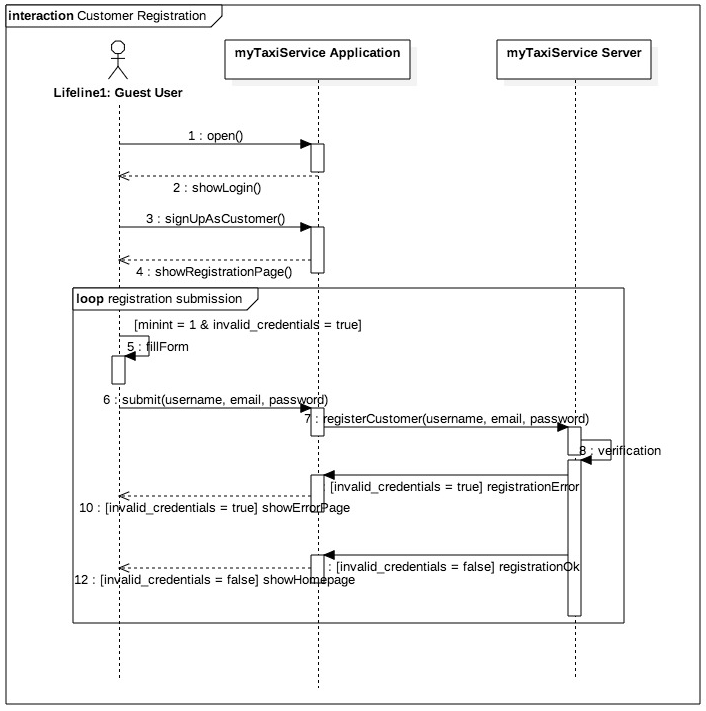
\includegraphics[width=\textwidth, scale=0.5]{IMG/InteractionDiagrams/CustomerRegistration_Normal.png}
					\caption{Customer Registration Interaction Diagram}\label{sec:FigureCustomerRegistration_Normal}
				\end{figure}

			\subsubsection{Registration using a Facebook account.}

	To accompany this diagram, read the Scenario \hyperref[sec:FacebookCustomerRegistrationScenario]{S.2}.

				\begin{table}[htpb]
					\centering
					\label{tab:FacebookCustomerRegistrationDiagramTable}
					\begin{tabularx}{\textwidth}{ll}
						\hline
						\hline
							\textbf{Subject}
						& 
							\textbf{Description}\\
						\hline
							Actors	       &  Guest User, myTaxiService Application, \\
							               &  myTaxiService Server, Facebook Login System\\
						\hline
							Preconditions  &  Guest User must not be already registered\\
						\hline
							Execution      &  1.~Guest User open the myTaxiService Application.\\
										   &  2.~Guest User taps on the "Log in with Facebook" button.\\
										   &  3.~myTaxiService Application calls Facebook Login API\\
										   &  4.~Facebook Login System makes his stuff\\
										   &  5.~Facebook Login System reply\\
										   &  6.~myTaxiService Application shows the result to the \\
										   &     Guest User\\
						\hline
							Postconditions &  The Guest User is now a Customer, he is registered in \\ 
										   &  the database and he's now logged in.\\
						\hline
							Exceptions     &  1.~The connection is lost or the Guest User doesn't complete\\ 
										   &     the registration clicking the button.\\
									
						\hline
						\hline
					\end{tabularx}
				\end{table}

				\begin{center}
					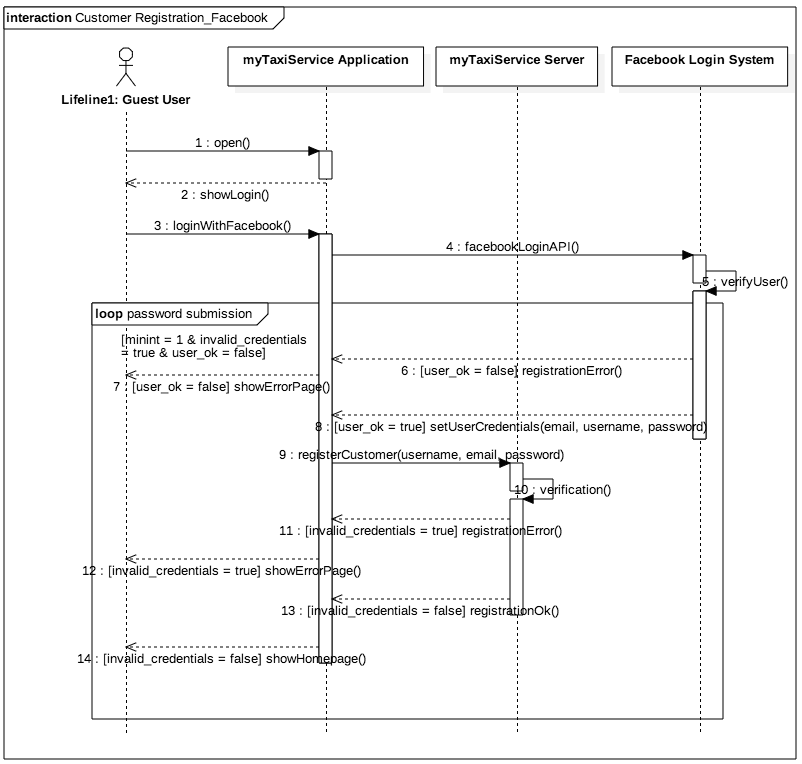
\includegraphics[scale=0.5]{IMG/InteractionDiagrams/CustomerRegistration_Facebook.png}
				\end{center}

			\subsubsection{Taxi Driver Registration}
			To accompany this diagram, read the Scenario \hyperref[sec:TaxiDriverRegistrationScenario]{S.3}.

				\begin{table}[htpb]
					\centering
					\label{tab:TaxiDriverRegistrationDiagramTable}
					\begin{tabularx}{\textwidth}{ll}
						\hline
						\hline
							\textbf{Subject}
						& 
							\textbf{Description}\\
						\hline
							Actors	       &  Guest User, myTaxiService Web Application, \\
										   &  myTaxiService Server\\
						\hline
							Preconditions  &  Guest User must not be already registered as a Taxi Driver\\
						\hline
							Execution      &  1.~Guest User open the myTaxiService Web Application.\\
										   &  2.~Guest User taps on the "Sign Up as a Taxi Driver" button.\\
										   &  3.~myTaxiService Web Application shows the registration page.\\
										   &  4.~Guest User fills up the registration form.\\
										   &  5.~Guest User taps on the "Submit" button.\\
										   &  6.~myTaxiService Web Application calls the server registration\\
										   &     service.\\
										   &  7.~myTaxiService Server verify the credentials\\
										   &  8.~myTaxiService Server reply with an ok or an error\\
										   &  9.~myTaxiService Web Application shows to the Guest User the\\
										   &     result of his registration.\\
						\hline
							Postconditions &  The Guest User is now a Taxi Driver, he is registered in \\ 
										   &  the database and he's now logged in.\\
						\hline
							Exceptions     &  1.~The email regex is not optimal (no regex for email is optimal)\\
										   &  2.~The connection is lost or the Guest User doesn't complete\\ 
										   &     the registration clicking the button.\\
									
						\hline
						\hline
					\end{tabularx}
				\end{table}
				
				\begin{centering}
					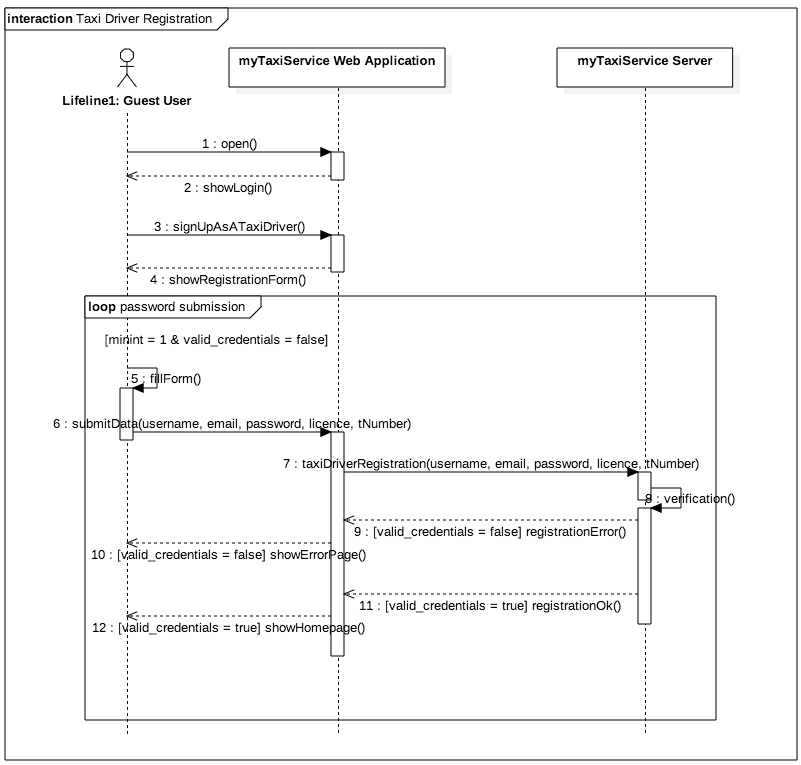
\includegraphics[scale=0.5]{IMG/InteractionDiagrams/TaxiDriverRegistration.png}
				\end{centering}

			\subsubsection{Registered User Login}
			To accompany this diagram, read the Scenario \hyperref[sec:RegisteredUserLoginScenario]{S.4}.

				\begin{table}[htpb]
					\centering
					\label{tab:RegisteredUserLoginDiagramTable}
					\begin{tabularx}{\textwidth}{lp{9cm}}
						\hline
						\hline
							\textbf{Subject}
						& 
							\textbf{Description}\\
						\hline
							Actors	       &  Guest User, myTaxiService Web Application, \\
										   &  myTaxiService Server\\
						\hline
							Preconditions  &  1.~Registered User must be registered on the system.\\
							               &  2.~Registered User must not be already logged in.\\
						\hline
							Execution      &  1.~Registered User opens the myTaxiService Web Application.\\
										   &  2.~Registered User fills the login form.\\
										   &  3.~Registered User presses on the "Login" button.\\
										   &  4.~myTaxiService Application submits the data to the server.\\
										   &  5.~myTaxiService Server checks the data.\\
										   &  6.~myTaxiService Server replies with an error or with success.\\
										   &  7.~myTaxiService Application shows an error notification or\\
										   &     a success one.\\
						\hline
							Postconditions &  The Registered User is now logged in and is able to use the\\
							               &  application.\\
						\hline
							Exceptions     &  1.~The connection is lost or the Guest User doesn't complete\\ 
										   &     the login clicking the button.\\
									
						\hline
						\hline
					\end{tabularx}
				\end{table}

				\begin{figure}[H]
					\centering
					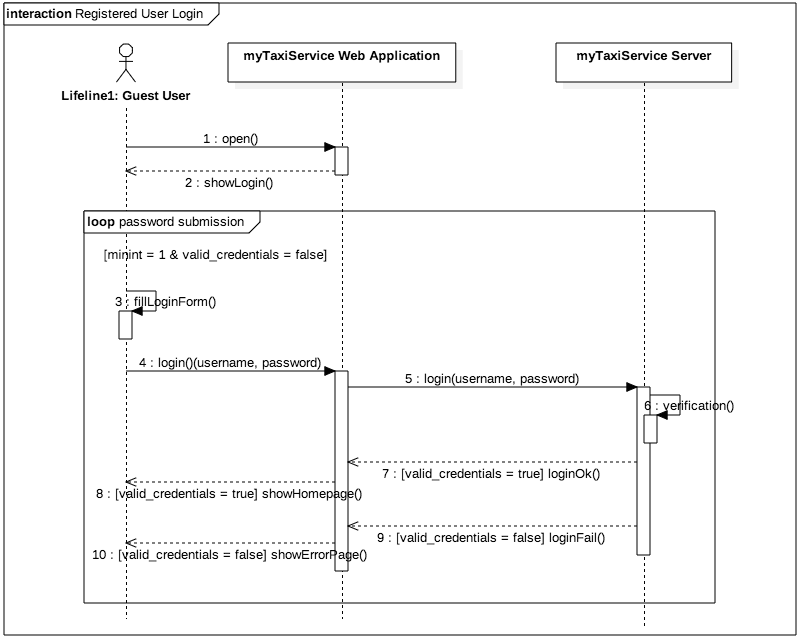
\includegraphics[width=\textwidth, scale=0.5]{IMG/InteractionDiagrams/RegisteredUserLogin.png}
					\caption{Login Interaction Diagram}\label{sec:FigureLogin}
				\end{figure}

			\subsubsection{Profile Modification}
			To accompany this diagram, read the Scenario \hyperref[sec:RegisteredUserProfileModificationScenario]{S.6}.

				\begin{table}[htpb]
					\centering
					\label{tab:RegisteredUserProfileModificationDiagramTable}
					\begin{tabularx}{\textwidth}{lp{9cm}}
						\hline
						\hline
							\textbf{Subject}
						& 
							\textbf{Description}\\
						\hline
							Actors	       &  Registered User, myTaxiService Web Application, myTaxiService Server\\
						\hline
							Preconditions  &  Registered User must be logged in.\\
						\hline
							Execution      &  1.~Registered User opens the myTaxiService Web Application.\\
										   &  2.~Registered User taps on the "Me" button.\\
										   &  3.~myTaxiService Web Application shows the profile page.\\
										   &  4.~Registered User changes his credentials.\\
										   &  5.~Registered User taps on the "Save" button.\\
										   &  6.~myTaxiService Web Application calls the server modification function.\\
										   &  7.~myTaxiService Server verifies the credentials\\
										   &  8.~myTaxiService Server replies with an ok or an error\\
										   &  9.~myTaxiService Web Application shows to the Registered User the result.\\
						\hline
							Postconditions &  Registered User's credentials are now changed.\\
						\hline
							Exceptions     &  1.~The Registered User disconnects before saving.\\
									
						\hline
						\hline
					\end{tabularx}
				\end{table}
				
				\begin{figure}[H]
					\centering
					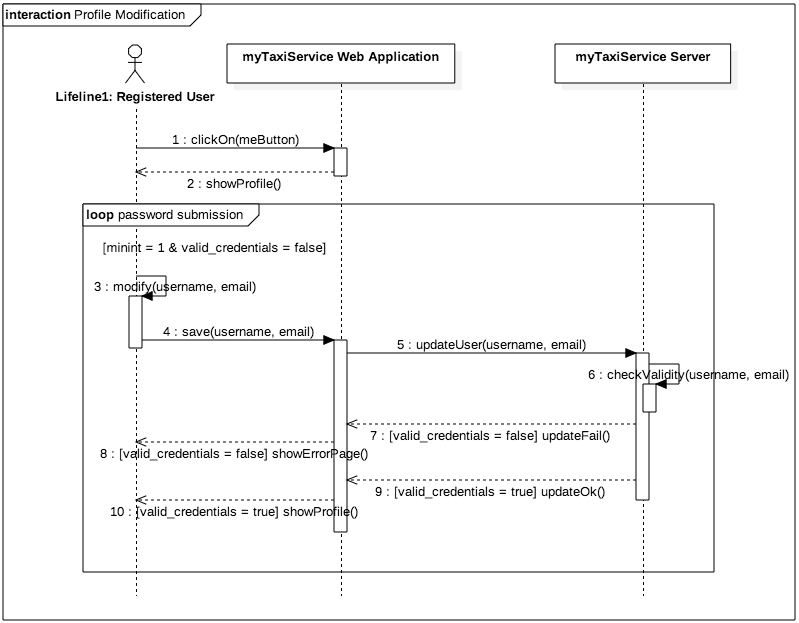
\includegraphics[width=\textwidth, scale=0.5]{IMG/InteractionDiagrams/ProfileModification.png}
					\caption{Profile Modification Interaction Diagram}\label{sec:FigureProfileModification}
				\end{figure}

			\subsubsection{Password Retreival}
			To accompany this diagram, read the Scenario \hyperref[sec:PasswordRetrievalScenario]{S.7}.

				\begin{table}[htpb]
					\centering
					\label{tab:PasswordRetrievalDiagramTable}
					\begin{tabularx}{\textwidth}{lp{9cm}}
						\hline
						\hline
							\textbf{Subject}
						& 
							\textbf{Description}\\
						\hline
							Actors	       &  Registered User, myTaxiService Web Application, myTaxiService Server\\
						\hline
							Preconditions  &  Registered User must be actually registered.\\
						\hline
							Execution      &  1.~Registered User open the myTaxiService Web Application.\\
										   &  2.~Registered User taps on the "Retrieve Password" link.\\
										   &  3.~myTaxiService Web Application shows the email field.\\
										   &  4.~Registered User inserts his email.\\
										   &  5.~Registered User taps on the "Retrieve" button.\\
										   &  6.~myTaxiService Web Application calls the password retrieval function.\\
										   &  7.~myTaxiService Server verify the email.\\
										   &  8.~myTaxiService Server reply with an ok or an error\\
										   &  9.~myTaxiService Web Application shows to the Registered User the result.\\
						\hline
							Postconditions &  The system has sent an email to the Registered User containing his password.\\
						\hline
							Exceptions     &  1.~The Registered User disconnects before clicking on the "Retrieve" button.\\
									
						\hline
						\hline
					\end{tabularx}
				\end{table}
				
				\begin{figure}[H]
					\centering
					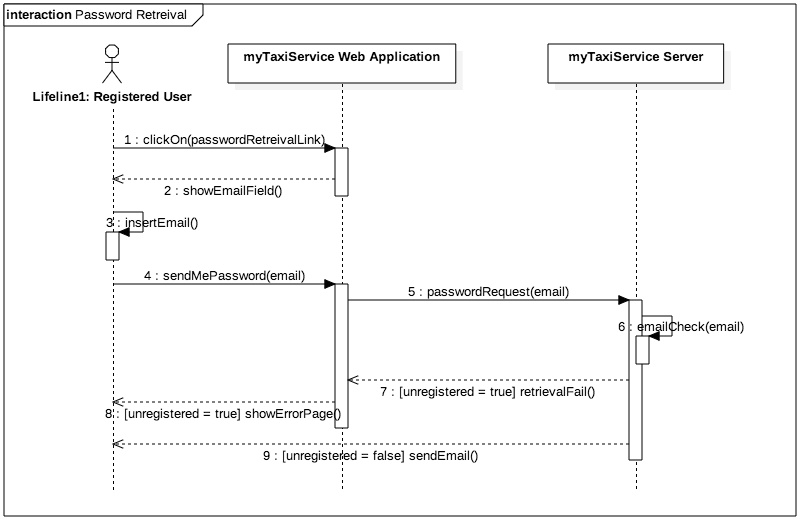
\includegraphics[width=\textwidth, scale=0.5]{IMG/InteractionDiagrams/PasswordRetrieval.png}
					\caption{Password Retrieval Interaction Diagram}\label{sec:FigureProfileModification}
				\end{figure}

			\subsubsection{Taxi Driver Reporting}
			To accompany this diagram, read the Scenario \hyperref[sec:TaxiDriverReportingScenario]{S.8}.

				\begin{table}[htpb]
					\centering
					\label{tab:TaxiDriverReportingDiagramTable}
					\begin{tabularx}{\textwidth}{lp{9cm}}
						\hline
						\hline
							\textbf{Subject}
						& 
							\textbf{Description}\\
						\hline
							Actors	       &  Customer, myTaxiService Mobile Application, myTaxiService Server\\
						\hline
							Preconditions  &  Customer must be logged in.\\
						\hline
							Execution      &  1.~Customer open the myTaxiService Mobile Application.\\
										   &  2.~Customer taps on the "Request Taxi" button.\\
										   &  3.~myTaxiService Mobile Application send the requests to the Server.\\
										   &  4.~Customer waits for the acceptance.\\
										   &  5.~myTaxiService Mobile Application shows the acceptance notification.\\
										   &  6.~Customer waits for the Taxi that does not arrive.\\
										   &  7.~Customer ends the ride reporting the Taxi Driver.\\
						\hline
							Postconditions &  The ride is set to ended and the Taxi Driver is reported.\\
						\hline
							Exceptions     &  1.~The Custoemr disconnects before reporting.\\
									
						\hline
						\hline
					\end{tabularx}
				\end{table}
				
				\begin{figure}[H]
					\centering
					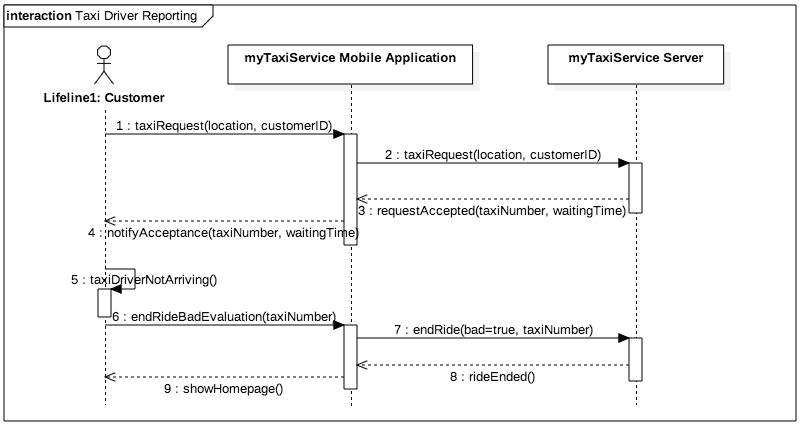
\includegraphics[width=\textwidth, scale=0.5]{IMG/InteractionDiagrams/TaxiDriverReporting.png}
					\caption{Taxi Driver Reporting Interaction Diagram}\label{sec:FigureTaxiDriverReporting}
				\end{figure}

			\subsubsection{Customer Reporting}
			To accompany this diagram, read the Scenario \hyperref[sec:CustomerReportingScenario]{S.8}.

				\begin{table}[htpb]
					\centering
					\label{tab:CustomerReportingDiagramTable}
					\begin{tabularx}{\textwidth}{lp{9cm}}
						\hline
						\hline
							\textbf{Subject}
						& 
							\textbf{Description}\\
						\hline
							Actors	       &  Taxi Driver, myTaxiService Mobile Application, myTaxiService Server\\
						\hline
							Preconditions  &  Taxi Driver must be logged in.\\
						\hline
							Execution      &  1.~Taxi Driver opens the myTaxiService Mobile Application.\\
										   &  2.~Taxi Driver receives a ride request notification from the Application.\\
										   &  3.~Taxi Driver accepts the ride request.\\
										   &  4.~Taxi Driver goes to the meeting location and the Customer is not there.\\
										   &  5.~Taxi Driver ends the ride reporting an abuse.\\
						\hline
							Postconditions &  The ride is set to 'ended' and the Customer is reported.\\
						\hline
							Exceptions     &  1.~The Taxi Driver disconnects before reporting.\\
									
						\hline
						\hline
					\end{tabularx}
				\end{table}
				
				\begin{figure}[H]
					\centering
					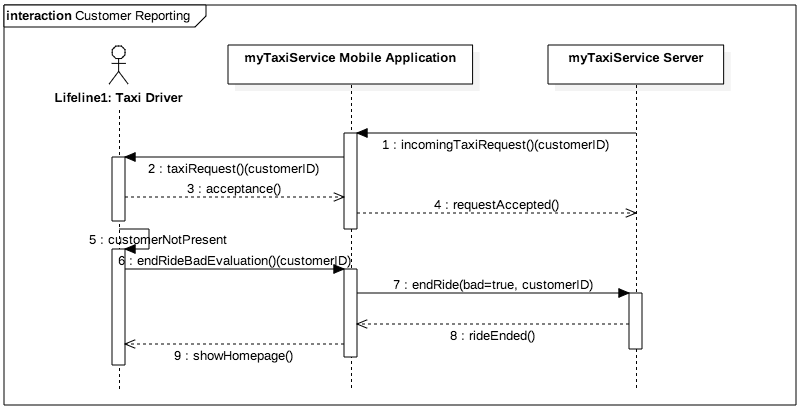
\includegraphics[width=\textwidth, scale=0.5]{IMG/InteractionDiagrams/CustomerReporting.png}
					\caption{Customer Reporting Interaction Diagram}\label{sec:FigureCustomerReporting}
				\end{figure}

		\subsection{State Machine Diagrams}

	%Non Functional Requirements Section
	\section{Non Functional Requirements}

		\subsection{Performance Requirements}

		\subsection{Design Constraints}

		\subsection{Software System Attributes}

			\subsubsection{Availability}

			\subsubsection{Maintainability}

			\subsubsection{Portability}

		\subsection{Security}

			\subsubsection{External Interface Side}

			\subsubsection{Application Side}

			\subsubsection{Server Side}
	\chapter{Appendix}
	
	\section{Alloy}
	This section is intended to present a model of the system and his constraints using the Alloy modeling language. We have divided the Alloy code in four main sections:
		\begin{itemize}
			\item Signatures, here are modeled the entities of our system. In the firs part there are primitive entities like boolean or strings and in the second part there are the system entities.
			\item Facts, here are modeled all the constraints for our model.
			\item Predicates and Assertions, here are modeled all the checks to control the consinstency of our model.
			\item Generated World, here there is an example of entities of our system generated by the "show" predicate in the Predicates and Assertions section.
		\end{itemize}

		\subsection{Signatures}
		Here there are attached screenshots of the Alloy code about entities:

				\begin{figure}[H]
					\centering
					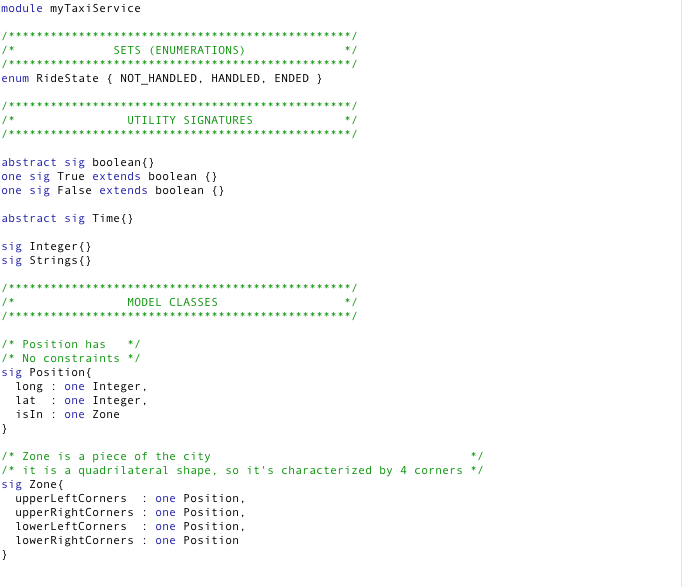
\includegraphics[width=\textwidth, scale=0.5]{IMG/ALLOY/SIG_1.png}
					\caption{Signatures 1}\label{sec:FigureSignatures1}
				\end{figure}

				\begin{figure}[H]
					\centering
					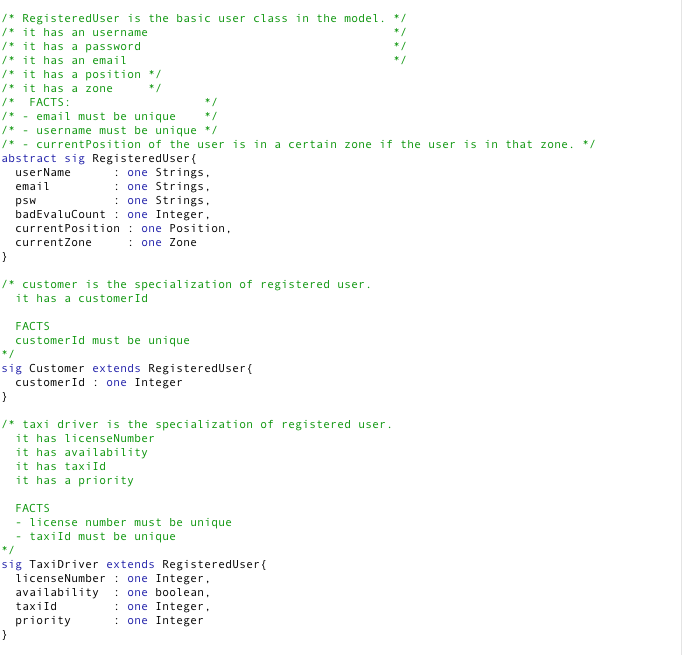
\includegraphics[width=\textwidth, scale=0.5]{IMG/ALLOY/SIG_2.png}
					\caption{Signatures 2}\label{sec:FigureSignatures2}
				\end{figure}

				\begin{figure}[H]
					\centering
					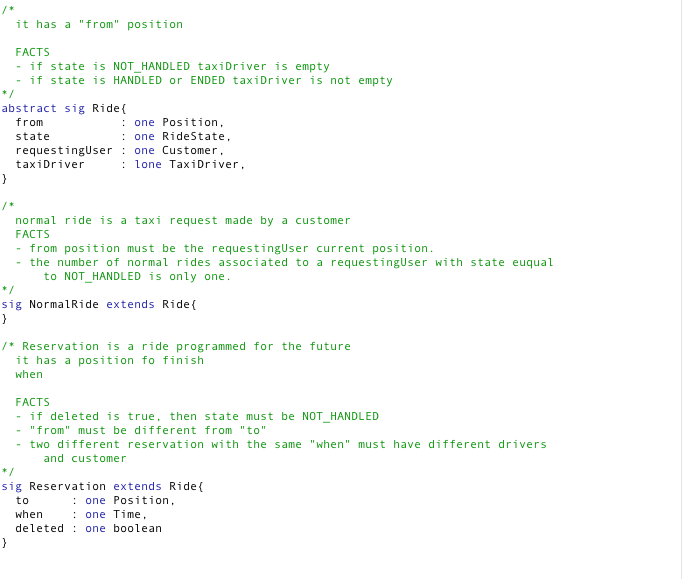
\includegraphics[width=\textwidth, scale=0.5]{IMG/ALLOY/SIG_3.png}
					\caption{Signatures 3}\label{sec:FigureSignatures3}
				\end{figure}

		\subsection{Facts}
		Here there are attached screenshots of the Alloy code about rules:

				\begin{figure}[H]
					\centering
					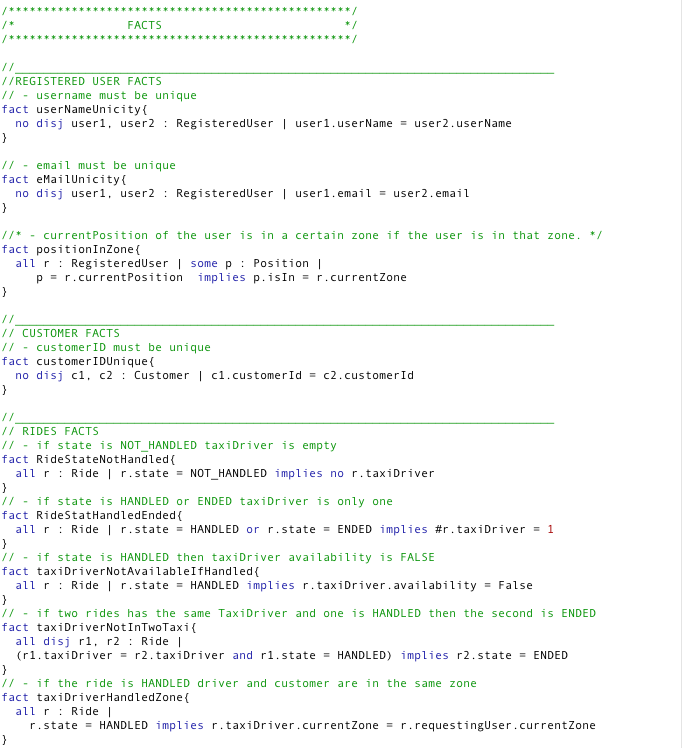
\includegraphics[width=\textwidth, scale=0.5]{IMG/ALLOY/FACT_1.png}
					\caption{Facts 1}\label{sec:FigureFacts1}
				\end{figure}

				\begin{figure}[H]
					\centering
					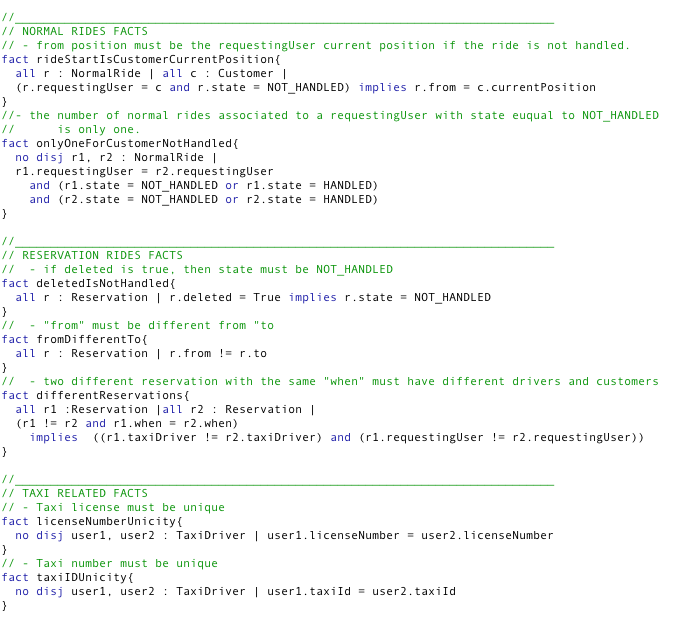
\includegraphics[width=\textwidth, scale=0.5]{IMG/ALLOY/FACT_2.png}
					\caption{Facts 2}\label{sec:FigureFacts2}
				\end{figure}

		\subsection{Predicates and Assertions}
		Here there are attached screenshots of the Alloy code about checks:

				\begin{figure}[H]
					\centering
					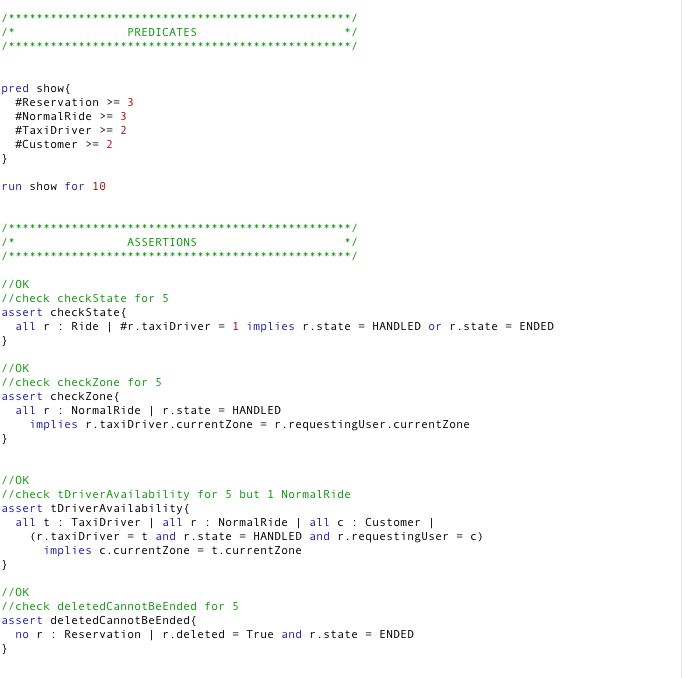
\includegraphics[width=\textwidth, scale=0.5]{IMG/ALLOY/PREN_ASS.png}
					\caption{Predicates and Assertions 1}\label{sec:FigureSignatures1}
				\end{figure}

		\subsection{Generated World}
		Here is the attached a screenshot of the entities generated by the "show" predicate:

				\begin{figure}[H]
					\centering
					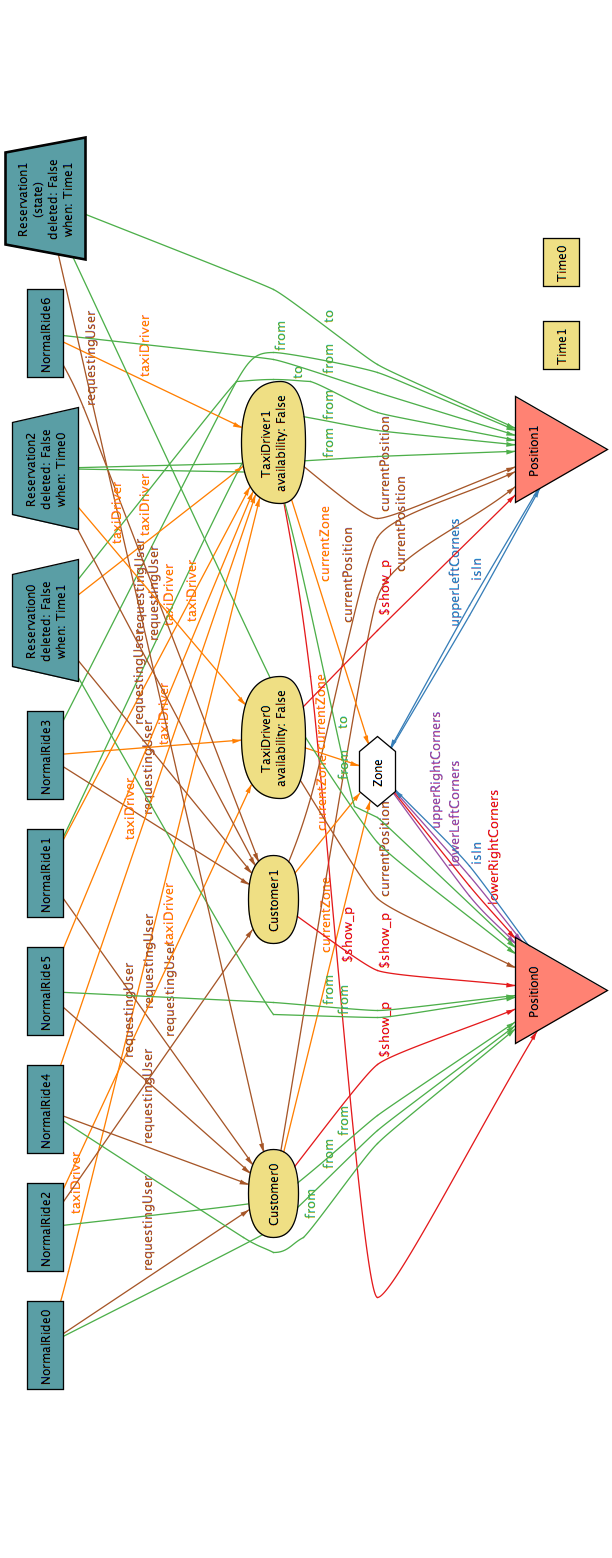
\includegraphics[width=\textwidth, height=\textheight, scale=0.5]{IMG/ALLOY/alloyWorld.png}
					\caption{Alloy World 1}\label{sec:FigureAlloyWorld1}
				\end{figure}		

	\section{Software and Tools}
To create this document we have used some common software:
	\begin{itemize}
		\item StarUML (\href{http://staruml.io}{link}) used to create UML models.
		\item Alloy Analyzer 4.2 (\href{http://alloy.mit.edu/alloy/index.html}{link}) used to model our system with Alloy language.
		\item Balsamiq Mockups (\href{http://balsamiq.com/products/mockups/}{link}) used to create mockups images.
	\end{itemize}

To write LaTeX code, we have used different software:
	\begin{itemize}
		\item Simone Deola: TexShop, provided with the MacTex package (\href{https://tug.org/mactex/}{link})
		\item Davide Cremona: Sublime Text editor (\href{http://www.sublimetext.com}{link}) with LaTeXTools (\href{https://github.com/SublimeText/LaTeXTools}{link}) and the Basic Package of MacTex (\href{https://tug.org/mactex/}{link})
	\end{itemize}

	\section{Hours of Work}


\end{document}